\documentclass[9pt]{beamer}
% \documentclass[notes, handout, 9pt]{beamer}
% \documentclass[handout, 9pt]{beamer}

\usepackage{import}
\subimport{../}{preamble.tex}
\subimport{../}{beamer-theme.tex}

% Location for all figures / pictures
\graphicspath{{pictures/}{figures/}}

% % Figures inline
\usepackage{tikz}
\usepackage{pgfplots}
\usetikzlibrary{calc}
\usetikzlibrary{shapes.multipart}
\usetikzlibrary{decorations.pathreplacing}
\usetikzlibrary{arrows.meta}
\usepgfplotslibrary{fillbetween}

%--------------------------------------------------
% Presentation Information
%--------------------------------------------------
\title[Continuous Optimization]{Variable Metric and Quasi-Newton Methods}
\author[]{\textbf{Bart Van Parys}}
\date[]{Fall 2026}
%--------------------------------------------------

\begin{document}

\begin{frame}  

  \maketitle

  \vspace{-2em}
  
    \begin{center}
    \begin{tabular}{lll}
      Instructor : & \textbf{Bart Van Parys} & \textbf{(\href{mailto:mastermath@vanparys.xyz}{mastermath@vanparys.xyz})} \\
    \end{tabular}
  \end{center}
  
\end{frame}

\section{The Contradiction of Subgradient Methods}

\begin{frame}{What is a Gradient ?}

  Let $f : \Re^n\to\nRe$ be continuous, and $s\in\Re^n$.

  \vfill

  \begin{itemize}
    \setlength\itemsep{1.5em}
  \item The function $f(x)$ is \emph{differentiable} at $x \in \dom(f)$ in direction $s$ if the following limit exists:
    \[
      \nabla f(x) [s] \defn \lim_{t\downarrow 0} \frac{f(x+t s)-f(x)}{t}
    \]
    and if $s\to \nabla f(x) [s]$ is linear (\emph{G\^ateaux differentiable}).
  \item The \emph{gradient} of $f$ at $x$ is the vector $f'(x)$ satisfying $\iprod{f'(x)}{s} = \nabla f(x) [s]$ for a
    \emph{particular scalar product} $\iprod{\cdot}{\cdot} : \Re^n\times\Re^n\to\Re$.
  \item The gradient depends \emph{arbitrarily} on the particular scalar product considered. No particular product is initially more justified than any other.
  \end{itemize}
  
\end{frame}

\begin{frame}{The Contradiction of Gradient Descent}

  \begin{center}
    \begin{tcolorbox}[width=0.5\textwidth]
      \[
        x_{k+1} \defn x_k - h_k f'(x_k).
      \]
    \end{tcolorbox}
  \end{center}

  \vfill
  
  Observation :
  \begin{itemize}
  \item $x_k$ is a point in $\Re^n$
  \item $f'(x_k)$ represents a linear function through a scalar product
  \end{itemize}

  \vfill
  
  \emph{It makes no sense to add them!} Akin to adding apples and oranges.
  
\end{frame}


\begin{frame} {Is the Canonical Basis Always the Best ?}

  Suppose that the feasible set $Q$ of your optimization problem is a diamond.

  \vfill
  
  \begin{center}
    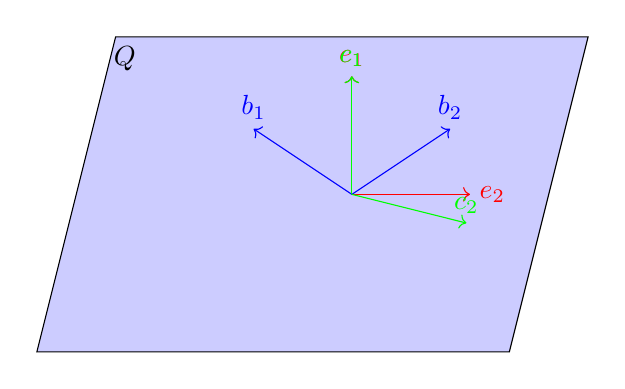
\begin{tikzpicture}

      
      \node (c1) at (-3, 2) {};
      \node (c2) at (3, 2) {};
      \node (c3) at (2, -2) {};
      \node (c4) at (-4, -2) {};

      \draw[fill=blue!20] (c1.center) node[below] {$~~Q$} -- (c2.center) -- (c3.center) -- (c4.center) -- cycle;

      \node (o) at (0, 0) {};

      \draw<1>[red, ->] (o.center) -- (0, 1.5) node[above] {$e_1$};
      \draw<1>[red, ->] (o.center) -- (1.5, 0) node[right] {$e_2$};

      \draw<1>[blue, ->] (o.center) -- ($0.416*(c1.center)$) node[above] {$b_1$};
      \draw<1>[blue, ->] (o.center) -- ($0.416*(c2.center)$) node[above] {$b_2$};

      \draw<2->[green, ->] (o.center) -- (0, 1.5) node[above] {$c_1$};
      \draw<2->[green, ->] (o.center) -- (1.455, -0.364) node[above] {$c_2$};

    \end{tikzpicture}

  \end{center}

  \vfill
  
  Naturally, the \blue{blue} basis is the more \blue{natural} than the \red{canonical} one.
  \uncover<2->{However, the green one is the most natural. The set $Q$ becomes a box.}
  
\end{frame}

\begin{frame}{Is Euclidean Distance Always Natural ?}

  \textbf{Example:} optimizing over probability vectors
  \[
    \begin{array}{rl}
      \inf & f(x) \\[0.5em]
      \st & x \in \Re_+^n, \\[0.5em]
           & \mb 1\tpose x = 1
    \end{array}
  \]

  \vfill

  \textbf{Remarks:}
  \begin{itemize}
  \item Euclidean distance is in general not recommended for measuring distance between probability vectors
  \item Statisticians indeed prefer Kullback-Leibler divergence, total variation distance, $\chi^2$-divergence, \dots
  \end{itemize}
  
  
\end{frame}

\begin{frame}{KL divergence}

  \begin{center}
    \includegraphics[height=5cm]{probability-divergence/probability-divergence.pdf}
  \end{center}

  \vfill

  KL-divergence
  \[
    D(p, q) = \sum_{i=1}^n( p_i \log(p_i/q_i) - p_i + q_i)
  \]
\end{frame}


\section{Mirror Descent}

\begin{frame}{Proximal Interpretation of Gradient Descent}

  \begin{center}
    \includegraphics[height=4cm]{proximal-term/proximal-term.pdf}
  \end{center}
  
  Gradient descent:
  \[
    x_{k+1} = \arg\min_{x\in E} \, \underbrace{f(x_k) + \iprod{f'(x_k)}{x-x_k}}_{\red{linear~approx.}} + \underbrace{\frac{1}{2h_k}\norm{x-x_k}^2_2}_{\blue{proximal~term}}
  \]
  \begin{itemize}
  \item Proximal term is used to monitor discrepancy between $f$ and its first-order approximation.
  \end{itemize}    
  
\end{frame}


\begin{frame}{Mirror Descent}

  \begin{center}
    \includegraphics[height=4cm]{proximal-term/proximal-term.pdf}
  \end{center}
  

  Mirror descent:
  \[
    x_{k+1} = \arg\min_{x\in E} \, \underbrace{f(x_k) + \nabla f(x_k)[x-x_k]}_{\red{linear~approx.}} + \underbrace{\frac{1}{h_k} D(x, x_k)}_{\blue{proximal~term}}
  \]
  where $D$ is defined as the Bregman divergence
  \[
    D(x, y) = V(x) - V(y) - \nabla V(y)[x-y].
  \]
\end{frame}

\begin{frame}{Bregman Divergence}

  \begin{center}
    \includegraphics[height=4cm]{bregman/bregman.pdf}
  \end{center}

  \vfill
  
  Let $V$ be a differentiable strictly convex function $E\to\Re$. Then 
  \[
    D(x, y) = V(x) - V(y) - \nabla V(y)[x-y]
  \]
  is a \emph{Bregman divergence}.
  
\end{frame}

\begin{frame}{Bregman Divergence}

   Let $V$ be a differentiable strictly convex function $E\to\Re$. Then 
  \[
    D(x, y) = V(x) - V(y) - \nabla V(y)[x-y]
  \]
  is a \emph{Bregman divergence}.

  \vfill
  
  \begin{itemize}
  \item Shares a few similarities to squared Euclidean distance
  \item For $V(x)=\norm{x}^2_2/2$ we have $D(x, y) = \frac12\norm{y-x}_2^2$
  \item Locally quadratic (when twice differentiable)
    \[
      D(x, y) = \frac12\iprod{V''(x) (y-x)}{y-x} + \mc O(\norm{y-x}_2^3).
    \]
  \end{itemize}

  
\end{frame}

\begin{frame}{Mirror Descent : Equivalence}

  Mirror descent:
  \[
    x_{k+1} = \arg\min_{x\in E} \, \underbrace{f(x_k) + \nabla f(x_k)[x-x_k]}_{\red{linear~approx.}} + \underbrace{\frac{1}{h_k} D(x, x_k)}_{\blue{proximal~term}}
  \]
  with first-order necessary and sufficent optimality conditions
  \begin{align*}
    & \nabla f(x_{k}) + \frac{1}{h_k} (\nabla V(x_{k+1}) - \nabla V(x_k)) = 0 \\
    \iff & \nabla V(x_{k+1}) = \nabla V(x_k) - h_k \nabla f(x_k).
  \end{align*}

  \vfill

  \uncover<2->{
  Hence, \emph{Mirror Descent} can be simplified to
  \[
    \left\{
      \begin{array}{rl}
        s_{k+1} & = s_k- h_k \nabla f(x_k)\\[0.5em]
        x_{k+1} & = \nabla V^\star(s_{k+1})
      \end{array}
    \right.
  \]
  as $s_{k} = \nabla V(x_k) \iff x_k = \nabla V^\star(s_k)$.
  }
\end{frame}

\begin{frame}{The Mirror Descent Method}

  \begin{minipage}{0.5\textwidth}
    \begin{equation*}
      %\tag{$\mc P$}
      \min_{x\in E} ~f(x)
    \end{equation*}
  \end{minipage}%
  \hfill
  \begin{minipage}{0.5\textwidth}
    \begin{itemize}
    \item $f:E\to\Re$ is \emph{differentiable convex}
    \item Oracle : $x\mapsto (f(x), \nabla f(x))$
    \item Absolute accuracy $\epsilon$
    \end{itemize}
  \end{minipage}

  \vfill

  \begin{algorithm}[H]
    \SetKwInput{Initialization}{Initialisation}
    \Initialization{$x_0\in E$, $s_0\defn\nabla V(x_0) \in E^\star$}
    \For{$k\geq 0$}{
      $s_{k+1} \defn s_k - h_k \nabla f(x_k)$  \hfill{\rm{\gray{Gradient descent in $E^\star$}}}\\
      $x_{k+1} \defn \nabla V^\star(s_{k+1})$ \hfill{\rm{\gray{Map back to $E$}}}~\,
    }
    \caption{\emph{Mirror Descent Method}}
  \end{algorithm}

\end{frame}

\begin{frame}{Picture}
\end{frame}

\begin{frame}{The Mirror Descent Method Converges [$\star$]}

  Assume $V^\star$ is $\mc L$-smooth and $f$ is $L$-Lipschitz.

  \vfill

  \textbf{Convergence :} We use as potential $0 \leq \phi(s) \defn V^\star(s) - s(x^\star) + V(x^\star)$. We have
  \begin{align*}
    \phi(s_{k+1}) & = \phi(s_k-h_k \nabla f(x_k)) = V^\star(s_k-h_k\nabla f(x_k)) -s_k(x^\star) + h_k \nabla f(x_k)[x^\star] + V(x^\star) \\
                  & \leq V^\star(s_k) \!-\! h_k \nabla V^\star(s_k)[\nabla f(x_k)] \!+\! \frac{\mc L h_k^2}{2} \norm{\nabla f(x_k)}^2_\star \!-\! s_k(x^\star) \!+\! h_k \nabla f(x_k)[x^\star] \!+\! V(x^\star)\\
                  & = V^\star(s_k) - h_k \nabla f(x_k)[x_k] + \frac{\mc L h_k^2}{2} \norm{\nabla f(x_k)}^2_\star - s_k(x^\star) + h_k \nabla f(x_k)[x^\star]+V(x^\star) \\
                  & = \phi(s_k)- h_k \nabla f(x_k)[x_k-x^\star] + \frac{\mc L h_k^2}{2} \norm{\nabla f(x_k)}^2_\star.
  \end{align*}
  Using the gradient inequality $\nabla f(x_k)[x^\star-x_k]\leq f(x^\star)-f(x_k)$ we get
  \[
    h_k (f(x_k)-f(x^\star))\leq \phi(s_k) - \phi(s_{k+1}) + \frac{\mc L h_k^2}{2} \norm{\nabla f(x_k)}^2_\star.
  \]
  Let $f(\tilde x_N) = \min_{k\in [1, \dots, N]}~f(x_k)$.
  Summing up over $k\in[0, N]$ and assuming $\norm{\nabla f}_\star \leq L$:
  \[
    f(\tilde x_N) - f(x^\star) \leq \frac{\phi(s_0) + \sum_{k=0}^N h^2_k \mc L L^2/2 }{\sum_{k=0}^N h_k}.
  \]

\end{frame}

\begin{frame}{The Mirror Descent Method Converges}

  Essentially, the proof is the same as for the subgradient method.

  \begin{center}
    \begin{tcolorbox}
      \[
        f(\tilde x_N) - f(x^\star) \leq \frac{\phi(s_0) + \sum_{k=0}^N h^2_k \mc L L^2/2 }{\sum_{k=0}^N h_k}
      \]
    \end{tcolorbox}
  \end{center}

  %As $V^\star(s_{N+1}) \geq s_{N+1}(x^\star) - V(x^\star)$, if $V^\star(s_0)=0$ we can bound $\phi(s_0)-\phi(s_{N+1})$ by $V(x^\star)$.

  \vfill
  \textbf{Convergence} is ensured if $\sum_{k=0}^N h_k \to \infty$ and $\sum_{k=0}^N h_k^2 < c$ as $N\to \infty$. In practice, these methods can be much faster than standard subgradient methods.

\end{frame}

\section{Example : Distributional Optimization}

\begin{frame}{Example : Optimization over Distributions}

  \textbf{Example:} optimize over all probability vectors
  \[
    \begin{array}{rl}
      q= \arg\min & f(x) \\[0.5em]
      \st & x \in \Re_+^n, \\[0.5em]
           & \mb 1\tpose x = 1
    \end{array}
  \]
  the function
  \(
    f(x) = \sum_{i=1}^n \tfrac{(x_i-q_i)^2}{q_i}
  \)
  with $q> 0$ and $\mb 1\tpose q = 1$.

  \vfill

  \textbf{Remarks:}
  \begin{itemize}
  \item Gradient has components
    \(
      f_i'(x) = 2 (\tfrac{x_i}{q_i}-1)
    \)
  \item Hessian is diagonal with
    \(
      f_{ii}''(x) = \tfrac{2}{q_i}
    \)
  \item Objective function $f$ is hence $L=\max_{i}\tfrac{2}{q_i}$-smooth and $\mu=\min_i\tfrac{2}{q_i}$-strongly convex.
  \end{itemize}
\end{frame}

\begin{frame}{Example : Gradient Descent}

  Projected gradient descent:
  \[
    x_{k+1} = \pi_Q(x_k - \tfrac{2 f'(x_k)}{(\mu+L)} )
  \]
  \begin{itemize}
  \item Exercise: find closed form formula for $\pi_Q$
  \end{itemize}
  
  \vfill

  \textbf{Theorem  (Nesterov):} We have that for $f$ $L$-smooth and $\mu$-strongly convex
  \[
    f(x_k) - f^\star \leq \frac L2 \left(\frac{C-1}{C+1}\right)^{2k} \norm{x_0-x^\star}^2
  \]
  with $C=\tfrac L\mu$.
\end{frame}

\begin{frame}{Example : Accelerated Gradient Descent}

  Projected accelerated gradient descent:
  \begin{align*}
    x_{k+1} & = \pi_Q(y_k - \tfrac{2 f'(y_k)}{(\mu+L)} )\\[0.5em]
    y_{k+1} & = x_{k+1} + \frac{\sqrt{L}-\sqrt{\mu}}{\sqrt{L}+\sqrt{\mu}} (x_{k+1}-x_k)
  \end{align*}

  
  \vfill

  \textbf{Theorem  (Nesterov):} We have that for $f$ $L$-smooth and $\mu$-strongly convex
  \[
    f(x_k) - f^\star \leq \min\{ (1-\tfrac {1}{\sqrt{C}})^k, \frac{4L}{(2\sqrt{L}+k\sqrt{\mu})^2} \} \cdot\left[(f(x_0)-f^\star)+ \frac\mu 2 \norm{x_0-x^\star}^2\right]
  \]
  with $C=\tfrac L\mu$.
\end{frame}

\begin{frame}{Example : Comparison}

  \begin{center}
    \includegraphics[height=6.8cm]{gradient-convergence/gradient-convergence.pdf}
  \end{center}
  
\end{frame}

\begin{frame}{Example : Mirror Descent}

  \begin{itemize}
  \item     Use the mirror function $$V(x)=\begin{cases}\sum_{i=1}^n x_i \log(x_i) & {\rm{if~}} x\in \Re_+^n ~{\rm{and}}~ \sum_{i=1}^n x_i=1, \\ +\infty & {\rm{otherwise.}}\end{cases}$$
    
  \item Its implied Bregman divergence is
    \[
      D(x, y) = \sum_{i=1}^n( x_i \log(x_i/y_i) - x_i + y_i)
    \]
    precisely the KL divergence. (See exercise 3.12 in Boyd and Vandenberghe)
  \item Its conjugate satisfies 
    \[
      V^\star(s) = \log(\sum_{i=1}^n \exp(s_i)) \quad {\rm{and}} \quad V^{\star'}_i(s) = \frac{\exp(s_i)}{\sum_{i=1}^n \exp(s_i)}.
    \]
  \end{itemize}

\end{frame}

\begin{frame}{Example : Entropic Descent Method}

  Entropic descent method:
  \begin{align*}
      s_{k+1} & = s_k - h_k f'(x_k)  \\[0.5em]
      x_{k+1, i} & = \frac{\exp(s_{k+1,i})}{\sum_{i=1}^n \exp(s_{k+1, i})}
  \end{align*}
\end{frame}

\begin{frame}{Example : Comparison}

  \begin{center}
    \includegraphics[height=6.8cm]{mirror-convergence/mirror-convergence.pdf}
  \end{center}
  
\end{frame}

\section{Quasi Newton Methods}

\begin{frame}{Using the Best Quadratic Approximation : Newton Method}

  Recall the reformulation of the gradient method
  \[
    x_{k+1 } \in \arg \min_{x} f(x_k) + \iprod{f'(x_k)}{x-x_k} + \frac{1}{2 h_k} \norm{x - x_k}^2_2. 
  \]

  Consider
  \[
    x_{k+1 } \in \arg \min_{x} f(x_k) + \iprod{f'(x_k)}{x-x_k} + \frac{1}{2} \iprod{f''(x_k)(x - x_k)}{x - x_k}
  \]
  in which we substituted the matrix $\mb I_n/h_k$ with the Hessian $f''(x_k)$.

  \vfill

  \emph{Newton's Method :}
  \begin{center}
    \begin{tcolorbox}[width=0.7\textwidth]
      \[
        x_{k+1} \defn x_k - f''(x_k)^{-1} f'(x_k)
      \]
    \end{tcolorbox}
  \end{center}

\end{frame}


\begin{frame}{Newton's Method Has Disadvantages}

  \begin{itemize}
    \setlength\itemsep{1em}
  \item Oracle : $x\mapsto (f(x), f'(x) , f''(x))$
  \item The Hessian should be invertible
  \item As such not applicable to constrained problems
  \item Expensive if $f''(x)$ is a dense matrix
  \end{itemize}

  \vfill

  What about the \emph{convergence} ?
  
\end{frame}

\begin{frame}{Convergence is much faster}

  \begin{minipage}{0.7\textwidth}
    Let $f:\Re^n\to\nRe$ satisfy
    \begin{itemize}
      \setlength\itemsep{1em}
    \item $f$ is twice differentiable
    \item $f''(x^\star) \succeq_{S^n_+} \ell \cdot \mb I_n \succ 0$
    \item The Hessian $f''$ is Lipschitz continuous w.r.t.\ $\norm{\cdot}_2$, i.e.,
      \[
        \norm{f''(x) -f''(y)}_2\leq M \norm{x-y}_2
      \]
      where $\norm{A} = \sup_{\norm{x}_2\leq 1} \norm{A x}_2 = \max_i \abs{\lambda_i(A)}$.
    \end{itemize}    
  \end{minipage}%
  \hfill
  \begin{minipage}{0.3\textwidth}
    \centering
    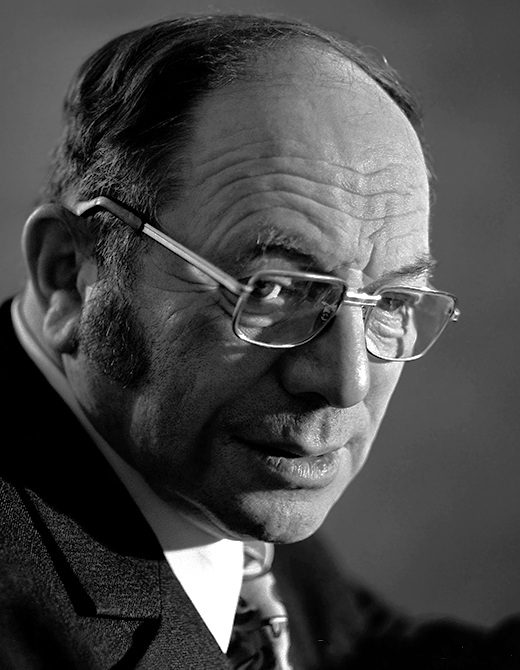
\includegraphics[height=3cm]{kantorovich.jpg}\\
    Kantorovich
  \end{minipage}

  \vfill
  
  \textbf{Theorem :} If $\norm{x_0-x^\star}_2 \leq \frac{2\ell}{3 M}$, then the iterates $x_k$ of Newton's method are \emph{well-defined} and
  \[
    \norm{x_{k+1}-x^\star}_2 \leq \frac{M \norm{x_k-x^\star}_2^2}{2 \left( \ell - M \norm{x_k-x^\star}_2\right)}\leq \frac{3M}{2 \ell} \norm{x_k-x^\star}_2^\emph{2}.
  \]
  
\end{frame}

\begin{frame}{Convergence Speed}

  \begin{itemize}
  \item Gradient / Mirror descent has linear convergence:
    \[
      \lim_{k\to \infty} \frac{\norm{x_{k+1}-x^\star}}{\norm{x_{k}-x^\star}} \in (0, 1).
    \]
  \item<2-> Newton method has quadratic convergence:
    \[
      \lim_{k\to \infty} \frac{\norm{x_{k+1}-x^\star}}{\norm{x_{k}-x^\star}^{\blue{2}}} \in (0, \infty).
    \]
  \item<3-> Quasi Newton methods are first-order methods with superlinear convergence
    \[
      \lim_{k\to \infty} \frac{\norm{x_{k+1}-x^\star}}{\norm{x_{k}-x^\star}} = 0.
    \]
  \end{itemize}
  

\end{frame}

\begin{frame}{Quasi-Newton Methods}

  Consider
  \begin{align*}
    x_{k+1 } = & \arg \min_{x} f(x_k) + \iprod{f'(x_k)}{x-x_k} + \frac{1}{2} \iprod{H_k(x - x_k)}{x - x_k} \\
     = & x_k - H_k^{-1}  f'(x_k)
  \end{align*}
  in we think of $H_k$ as an approximation of the Hessian $f''(x_k)$.

  \vfill

  Construction of $H_k\in \S^n_{++}$ should
  \begin{itemize}
  \item Avoid second derivatives
  \item Simplify computation of search direction
  \end{itemize}  
  
\end{frame}

\begin{frame}{Descent Direction}

  \textbf{Observation:} If $H_{k}\in \S^n_{++}$ then Newton direction $d_{k} = -H_k^{-1}f'(x_k)$ is a descent direction, i.e.,
  \[
    \iprod{f'(x_k)}{d_k} = -\langle f'(x_k), H_k^{-1}f'(x_k)\rangle < 0.
  \]


\end{frame}

\begin{frame}{Quasi-Newton Methods}

  \begin{algorithm}[H]
    \SetKwInput{Initialization}{Initialisation}
    \Initialization{$x_0\in \Re^n$, $H_0\in S^n_+$}
    \For{$k\geq 0$}{
      Search direction
      \[
        d_{k} = -H_k^{-1} f'(x_k)
      \]\\
      Determine step size $t_k$ using Wolfe-conditions\\
      Step
      \[
        x_{k+1} = x_k + t_k d_k
      \]\\
      Compute approximate Hessian $H_{k+1}$
    }
    \caption{\emph{Quasi-Newton Method}}
  \end{algorithm}

  \vfill
  
  \textbf{Remarks:}
  \begin{itemize}
  \item Different update rules for $H_{k+1}$
  \item Avoid extra computation by working with $H_{k+1}^{-1}$ directly
  \end{itemize}
\end{frame}

\begin{frame}{BFGS Update}

  Approximate Hessian update
  \[
    H_{k+1} = H_k + \frac{y_k y_k\tpose}{y_k\tpose d_k} - \frac{H_k d_k d_k\tpose H_k}{d_k\tpose H_k d_k} 
  \]
  with $y_k = f'(x_{k+1})-f'(x_k)$ and $y_k\tpose d_k>0$ for strictly convex $f$.

  \vfill

  Approximate Inverse Hessian update
  \[
    H^{-1}_{k+1} = \left(\mb I - \frac{d_ky_k\tpose}{y_k\tpose d_k}\right) H^{-1}_k \left(\mb I - \frac{y_k d_k\tpose}{y_k\tpose d_k}\right) + \frac{d_k d_k\tpose}{y_k\tpose d_k} 
  \]
\end{frame}

\begin{frame}{Secant Condition}

  The BFGS update satisfies the \emph{secant condition}
  \[
    H_{k+1} d_k = f'(x_{k+1})-f'(x_k)
  \]

  \vfill
  
  \textbf{Interpretation:} the quadratic model
  \[
    m(x_{k+1}) = f(x_{k+1}) + \iprod{f'(x_{k+1})}{x-x_{k+1}} + \iprod{H_{k+1}(x-x_{k+1})}{x-x_{k+1}}/2
  \]
  around $x_{k+1}$ has correct gradients at previous two iterates.

  \vfill
  
  \begin{itemize}
  \item By construction $m'(x_{k+1}) = f'(x_{k+1})$
  \item Secant condition implies that
    \begin{align*}
      m'(x_k) & = f'(x_{k+1})+H_{k+1}(x_k-x_{k+1}) \\[0.5em]
              & = f'(x_k).
    \end{align*}
  \end{itemize}
  
\end{frame}

\begin{frame}{Least Change Updates}

  Most families of update rules can be interpreted as
  \[
    \begin{array}{rl}
      H_{k+1} = {\displaystyle \min_{X\succ 0}} & D(X, H_k) \\[0.5em]
      \st & X d_k = f'(x_{k+1})-f'(x_k).
    \end{array}
  \]

  \vfill
  \textbf{Remarks:}
  \begin{itemize}
  \item Distance function $D:S_{++}^n\times S^{n}_{++}\to \Re_+$.
  \end{itemize}

\end{frame}


\begin{frame}{Optimality of BFGS Update}

  The BFGS update can be defined as
  \[
    \begin{array}{rl}
      H_{k+1} = {\displaystyle \min_X} & \tr ( H_k^{-1} X ) - \log \det ( H_k^{-1} X ) \\[0.5em]
      \st & X d_k = f'(x_{k+1})-f'(x_k).
    \end{array}
  \]
  \begin{itemize}
  \item BFGS update is a least-change secant update
  \end{itemize}

\end{frame}

\begin{frame}{DFP Update}

  The DFP update can be defined as
  \[
    \begin{array}{rl}
      H_{k+1} = {\displaystyle \min_X} & \tr ( H_k X ^{-1} ) - \log \det ( H_k X ^{-1} ) \\[0.5em]
      \st & X d_k = f'(x_{k+1})-f'(x_k).
    \end{array}
  \]
  \begin{itemize}
  \item DFP update is a least-change secant update
  \end{itemize}

  \vfill
  
  Explicit formula:
  \[
    H_{k+1} = \left(\mb I - \frac{yd_k\tpose}{d_k\tpose y}\right) H_k \left(\mb I - \frac{d_ky\tpose}{y\tpose d_k}\right) + \frac{y y\tpose}{d_k\tpose y } 
  \]
  predates the BFGS update but is less popular.
  
\end{frame}

\begin{frame}{Convergence}

  \textbf{Global Convergence:}
  If $f$ is strongly convex, BFGS with backtracking line search converges for any $x_0$

  \vfill

  \textbf{Local Speed:}
  If $f$ is strongly convex and $f''(x)$ is Lipschitz continuous, local convergence is superlinear:
  \[
      \lim_{k\to \infty} \frac{\norm{x_{k+1}-x^\star}}{\norm{x_{k}-x^\star}} = 0.
  \]
\end{frame}

\section{Example: Analytical Center}

\begin{frame}{Example : Analytical Center}
  \textbf{Example:} Analytical center of the probability simplex
  \[
    \begin{array}{rl}
      (1/n, \dots, 1/n)= \arg\min & f(x)=-\sum_{i=1}^n \log(x_i) \\[0.5em]
      \st & \mb 1\tpose x = 1
    \end{array}
  \]

  \vfill

  \textbf{Remarks:}
  \begin{itemize}
  \item Gradient has components
    \(
      f'(x) = -\tfrac{1}{x_i}
    \)
  \item Hessian is diagonal with
    \(
      f''(x) = \tfrac{1}{x_i^2}
    \)
  \end{itemize}

\end{frame}

\begin{frame}{Example : Newton Method with Equality Constraint}
  
  \begin{algorithm}[H]
    \SetKwInput{Initialization}{Initialisation}
    \Initialization{Feasible $x_0\in \Re^n$}
    \For{$k\geq 0$}{
      Search direction
      \[
        \begin{pmatrix} f''(x_k) & \mb 1 \\ \mb 1' & 0 \end{pmatrix} \begin{pmatrix} d_{k} \\ \lambda_{k} \end{pmatrix} = \begin{pmatrix} - f'(x_k)\\ 0 \end{pmatrix}
      \]\\
      Determine step size $t_k$ using Wolfe-conditions\\
      Step
      \[
        x_{k+1} = x_k + t_k d_k
      \]
    }
    \caption{\emph{Full-Newton Method}}
  \end{algorithm}

  \vfill

  \textbf{Remarks:}
  \begin{itemize}
  \item Full steps $t_k=1$ may cause divergence of Newton method
  \item Step-size rule using Wolfe-conditions ensures global convergence
  \end{itemize}
  
\end{frame}

\begin{frame}{Example : Quasi-Newton Method with Equality Constraint}

  \begin{algorithm}[H]
    \SetKwInput{Initialization}{Initialisation}
    \Initialization{$x_0\in \Re^n$, $H_0\in S^n_+$}
    \For{$k\geq 0$}{
      Search direction
      \[
        \begin{pmatrix} H_k & \mb 1 \\ \mb 1' & 0 \end{pmatrix} \begin{pmatrix} d_{k} \\ \lambda_{k} \end{pmatrix} = \begin{pmatrix} H_k x_k - f'(x_k)\\ 1 \end{pmatrix}
      \]\\
      Determine step size $t_k$ using Wolfe-conditions\\
      Step
      \[
        x_{k+1} = x_k + t_k d_k
      \]\\
      Compute approximate Hessian $H_{k+1}$ using BFGS
    }
    \caption{\emph{Quasi-Newton Method}}
  \end{algorithm}

\end{frame}

\begin{frame}{Example: Comparison}

  \begin{center}
    \includegraphics[height=6.8cm]{newton-convergence/newton-convergence.pdf}
  \end{center}  

\end{frame}

\end{document}
%%% Local Variables:
%%% mode: latex
%%% TeX-master: t
%%% End:
